\documentclass{beamer}
\usetheme{Boadilla}

\usepackage{amsmath}
\usepackage{amssymb}
\usepackage{amsfonts}
\usepackage{hyperref}
\usepackage{cancel}
\usepackage{multicol}
\usepackage{multirow}

\usepackage{amsmath}
\DeclareMathOperator*{\argmax}{arg\,max}
\DeclareMathOperator*{\argmin}{arg\,min}

\title[Fisher Matrix Approximation]{Approximate Fisher Information Matrix to Characterise the Training of Deep Neural Networks}
\author{Nikita Kiselev}
\institute{MIPT, 2024}


\begin{document}
\begin{frame}
    \titlepage
\end{frame}


\begin{frame}
    \tableofcontents
\end{frame}


\section{Motivation}
\begin{frame}{Motivation}
    \begin{block}{Main idea}
         Training of deep neural networks relies heavily on the careful selection of mini-batch sizes and learning rates. This selection process is often subjective and lacks clear guidelines. The proposed methodology use efficiently computed measures derived from the Fisher information matrix. These measures can help practitioners monitor and control the training process, leading to improved training convergence and generalization.
    \end{block} 
\end{frame}

\section{Definitions}
\begin{frame}{SGD objective}
    \begin{block}{Image Classification task}
        Given the dataset $\mathcal{D} = \{ \mathbf{x}_i, y_i \}_{i=1}^{|\mathcal{D}|}$, where the $i^{th}$ image $\mathbf{x}_i:\Omega \rightarrow \mathbb R$ is annotated with the label $y_i \in \{1,...,C\}$. This dataset is divided into training $\mathcal{T} \in \mathcal{D}$ and testing $\mathcal{S} \in \mathcal{D}$. The full model is defined by $f(\mathbf{x}, \theta )$, where $\theta \in \mathbb R^P$ denotes all model parameters. The objective is to minimise the multi-class cross entropy loss $\ell ( \cdot )$ on the training set $\mathcal{T}$, as follows:
        \begin{equation}
        \theta^* = \arg \min_{\theta} \frac{1}{|\mathcal{T}|}\sum_{i \in \mathcal{T}} \ell \left ( y_i , f(\mathbf{x}_i, \theta )  \right ).
        \end{equation}
    \end{block}
    \begin{block}{SGD}
        \begin{equation}
        \theta_{k+1} = \theta_{k} -   \frac{\alpha_k}{|\mathcal{B}_k|} \sum_{i \in \mathcal{B}_k} \nabla \ell(y_i,f(\mathbf{x}_i,\theta_k)),
        \label{eq:sgd}
        \end{equation}
        where $\mathcal{B}_k$ is the mini-batch for the $k^{th}$ iteration of the minimisation process.
    \end{block}
\end{frame}

\begin{frame}{Hessian matrix approximation}
    \begin{block}{Loss landscape shape}
        The shape of the loss function can be characterised by the spectrum of the $\nabla^2 \ell(y_i,f(\mathbf{x}_i,\theta_k))$, where sharpness is defined by the magnitude of the eigenvalues.
    \end{block}
    \begin{block}{Fisher information matrix}
        We define the Fisher information matrix as follows:
        \begin{equation}
        \mathbf{F}_k = \nabla \ell(y_{i \in \mathcal{B}_k},f(\mathbf{x}_{i \in \mathcal{B}_k},\theta_k))  \nabla \ell(y_{i \in \mathcal{B}_k},f(\mathbf{x}_{i \in \mathcal{B}_k},\theta_k))^{\top},
        \label{eq:F_k}
        \end{equation}
        where $\mathbf{F}_k \in \mathbb R^{P \times P}$. 
    \end{block}
    \begin{alertblock}{Idea}
        Fisher matrix can be a reasonable approximation of the Hessian matrix at the end of the training (assuming sufficient training has been done).
    \end{alertblock}
\end{frame}

\begin{frame}{Fisher matrix approximation}
    \begin{block}{Fisher matrix calculation}
        The calculation of $\mathbf{F}_k$ depends on the Jacobian $\mathbf{J}_k = \nabla \ell(y_{i \in \mathcal{B}_k},f(\mathbf{x}_{i \in \mathcal{B}_k},\theta_k))$, with $\mathbf{J}_k  \in \mathbb R^{P \times |\mathcal{B}_k|}$. 
    \end{block}
    \begin{alertblock}{Computational and memory complexity}
        Given that $\mathbf{F}_k = \mathbf{J}_k \mathbf{J}_k^{\top} \in \mathbb R^{P \times P}$ scales with $P \in [O(10^6),O(10^7)]$ and that we are only interested in the spectrum of $\mathbf{F}_k$, we can compute instead $\widetilde{\mathbf{F}}_k = \mathbf{J}_k^{\top} \mathbf{J}_k \in \mathbb R^{|\mathcal{B}_k| \times |\mathcal{B}_k|}$ that scales with the mini-batch size $|\mathcal{B}_k| \in [O(10^1),O(10^2)]$.  
    \end{alertblock}
    \begin{block}{Spectrum consistency}
        Note that the rank of $\widetilde{\mathbf{F}}_k$ and $\mathbf{F}_k$ is at most $|\mathcal{B}_k|$, which means that the spectra of $\widetilde{\mathbf{F}}_k$ and $\mathbf{F}_k$ are the same given that both will have at most $|\mathcal{B}_k|$ non-zero eigenvalues.
    \end{block}
\end{frame}

\section{Method}
\begin{frame}{Methodology}
    \begin{block}{1. Running average of the truncated condition number of $\widetilde{\mathbf{F}}_k$}
    \begin{equation}
    \bar{C}_K = \frac{1}{K}\sum_{k = 1}^K c_k, \quad c_k = \frac{\sigma_{\text{max}}(\widetilde{\mathbf{F}}_k)}{\sigma_{\text{min}}^+(\widetilde{\mathbf{F}}_k)}.
    \label{eq:cumsum_cond}
    \end{equation}
    \end{block}
    \begin{block}{2. Weighted cumulative sum of the energy of  $\widetilde{\mathbf{F}}_k$}
    \begin{equation}
    L_K  = \sum_{k = 1}^K l_k, \quad l_k  = \frac{\alpha_k}{|\mathcal{B}_k|} \left ( \mathrm{Tr} \left ( \widetilde{\mathbf{F}}_k \right ) \right )^{\frac{1}{2}}.
    \label{eq:cumsum_laplacian}
    \end{equation}
    \end{block}
    \begin{block}{3. Dynamic sampling}
    Change the mini-batch size during the training in order to achieve good convergence and generalisation.
    \end{block}
\end{frame}

\section{Experiments}
\begin{frame}{Experiments Setup}
    \begin{itemize}
        \item \textbf{Data:} CIFAR-10, CIFAR-100, SVHN, and MNIST.
        \item \textbf{Models:} ResNet and DenseNet.
        \item \textbf{Optimizer:} SGD with momentum of 0.9 and learning rate schedule as follows: $\times 0.1$ at the 50\% training epochs, and $\times 0.1$ at the 75\%.
        \item \textbf{Metric:} Accuracy on training and testing samples.
    \end{itemize}
\end{frame}

\begin{frame}{Mini-batch Size and Learning Rate}
    \begin{figure}
        \centering
        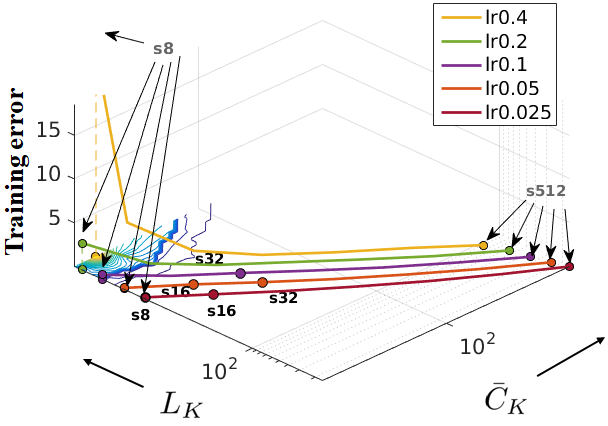
\includegraphics[width=0.45\textwidth]{figs/fig_batchsize_cifar10_train.png}
        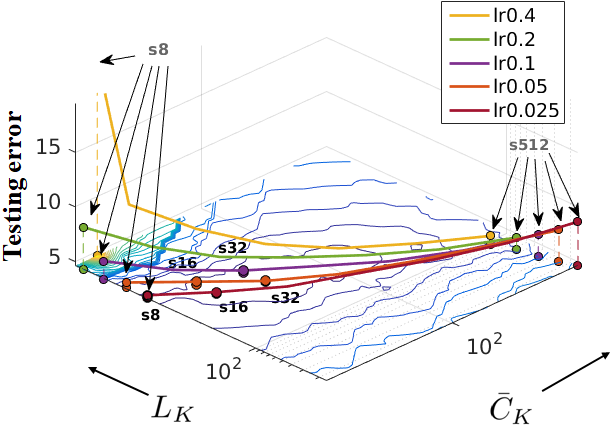
\includegraphics[width=0.45\textwidth]{figs/fig_batchsize_cifar10_test.png}
        \caption{ResNet on CIFAR-10. 1) Each configuration has a unique $\bar{C}_K$ and $L_K$ signature, where no configuration overlays over each other in the space;
        2) $|\mathcal{B}_k|$ is directly proportional to $\bar{C}_K$ and inversely proportional to $L_K$;
        3) $\alpha_k$ is directly proportional to $\bar{C}_K$ and $L_K$; and
        4) small $\bar{C}_K$ and large $L_K$ indicate poor training convergence, and large $\bar{C}_K$ and small $L_K$ show poor generalisation, so the best convergence and generalisation requires a small value for both measures.}
        \label{fig:batch-lr}
    \end{figure}
\end{frame}

\begin{frame}{Functional Relations for the Proposed Measures}
    \begin{figure}
        \centering
        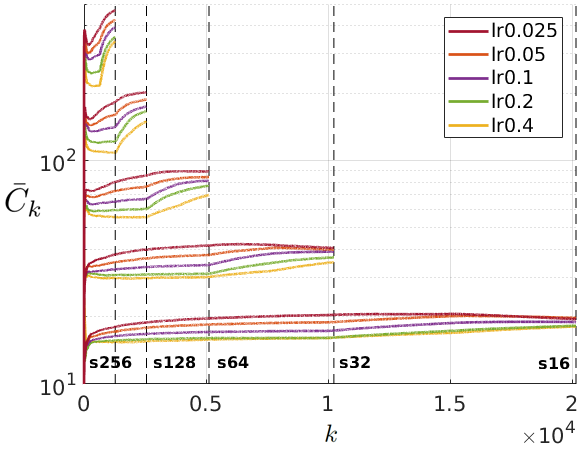
\includegraphics[width=0.45\textwidth]{figs/AVG_C_K_vs_iter.png}
        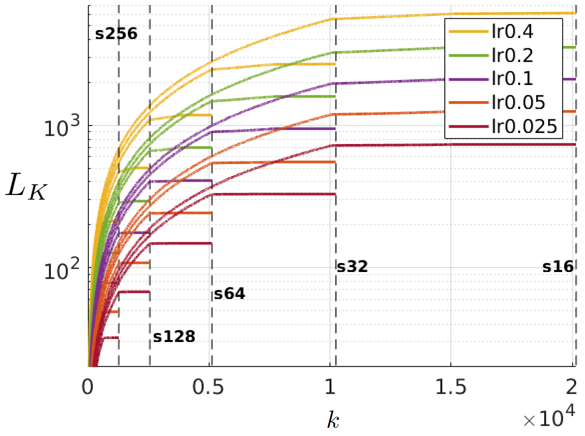
\includegraphics[width=0.45\textwidth]{figs/L_K_vs_iter.png}
        \caption{ResNet on CIFAR-10. 1) $\bar C_K$ tends to cluster at similar values for training processes performed with the same mini-batch sizes, independently of the learning rate; 2) $L_K$ is more likely to cluster at similar values for training processes performed with the same learning rate, independently of the mini-batch size, particularly at the first half of the training.}
        \label{fig:batch-lr}
    \end{figure}
\end{frame}

\begin{frame}{The stability of the proposed measures}
    \begin{figure}
        \centering
        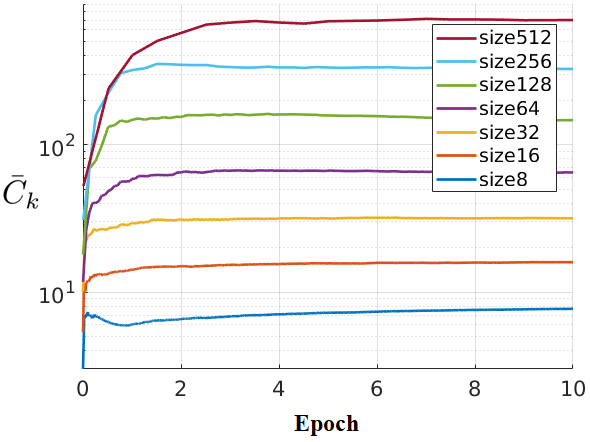
\includegraphics[width=0.45\textwidth]{figs/fig_batch_size_AVG_C_K_10epochs.png}
        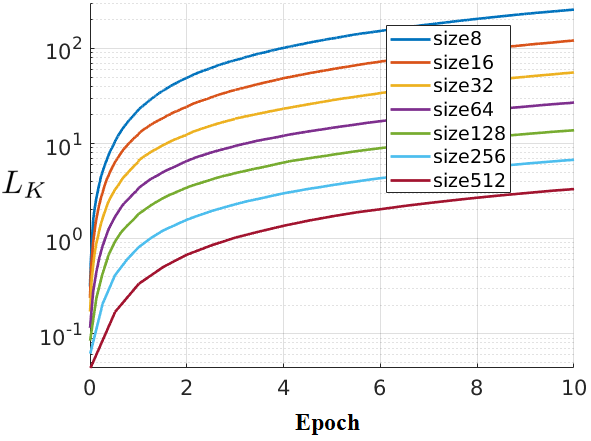
\includegraphics[width=0.45\textwidth]{figs/fig_batch_size_L_K_10epochs.png}
        \caption{ResNet on CIFAR-10. Proposed measures are stable in terms of the relative positions of $\bar{C}_K$ and $L_K$ values even during early training epochs.}
        \label{fig:batch-lr}
    \end{figure}
    \vspace{-0.5cm}
    \begin{alertblock}{Idea}
        Proposed $\bar{C}_K$ and $L_K$ values can be used to guide dynamic sampling~-- a method that dynamically increases the mini-batch size during the training, by navigating the training procedure in the landscape of $\bar{C}_K$ and $L_K$.
    \end{alertblock}
\end{frame}

\begin{frame}{Dynamic Sampling}
    \begin{columns}
    \begin{column}{0.45\textwidth}
        \begin{itemize}
            \item Divide the training process into five stages, each with equal number of training epochs and using a particular mini-batch size.
            \item $\bar{C}_K$ and $L_K$ are pushed away from the initial mini-batch size region towards the final mini-batch size region.
        \end{itemize}
    \end{column}
    \begin{column}{0.45\textwidth}
    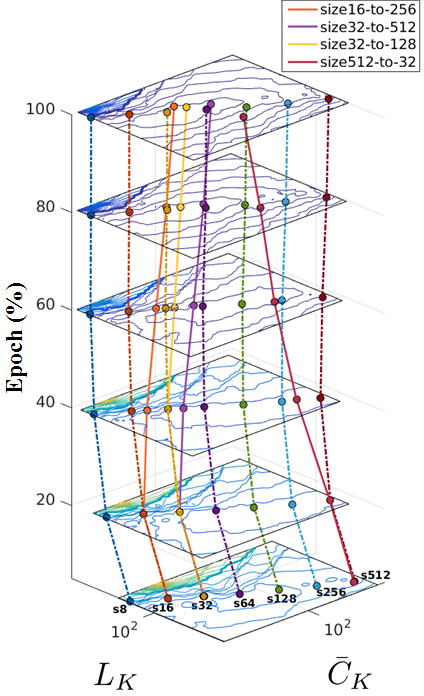
\includegraphics[width=0.8\textwidth]{figs/fig_dynamic_sampling_cifar10_test.png}
    \end{column}
    \end{columns}
\end{frame}

\begin{frame}{Comparison of different sampling strategies}
\begin{table}
\begin{center}
\resizebox{\textwidth}{!}{
\begin{tabular}{|c|l|c|c|c|}
\hline
& Model & \multicolumn{3}{c|}{CIFAR-10} \\ 
\cline{3-5}
& (best of each)  & {\bf s\#} & {\bf -$\emptyset$} & {\bf -MS} \\
\hline
\multirow{5}{*}{\rotatebox{90}{ResNet}} & Name & 
{\bf s32} & {\bf s32-to-128} & {\bf s32-to-128-MS} \\ 
\cline{2-5}
& Test Error & 
$4.78\% \pm 0.05\%$ & $4.90\% \pm 0.05\%$ & $4.76\% \pm 0.13\%$  \\
\cline{2-5}
& p-value vs {\bf s\#} & -- & 0.0048 & 0.72  \\
\cline{2-5}
& p-value {\bf -$\emptyset$} vs {\bf -MS} & -- & \multicolumn{2}{c|}{0.029} \\
\cline{2-5}
& Training Time (h) &
7.7 & 7.0 & 7.1  \\
\hline
\end{tabular}%
}
\end{center}
\caption{The comparison between the best "beacon" model {\bf s\#} (at {\bf lr0.1}), and the best dynamic sampling models {\bf -$\emptyset$}, and {\bf -MS}. The latter ({\bf -MS}) corresponds to sampling of mini-batch sizes over each different learning rate value.}
\label{table:dynamic_sampling}
\end{table}
\vspace{-0.5cm}
\begin{block}{Overview}
    In general, the results show that dynamic sampling allows a faster training and a similar classification accuracy, compared with the fixed sampling training of the beacons. 
\end{block}
\end{frame}

\section{Literature}
\begin{frame}{Literature}
    \begin{enumerate}
        \item \textbf{Main article:} \href{https://arxiv.org/abs/1810.06767}
        {Liao Z. et al. Approximate fisher information matrix to characterize the training of deep neural networks // IEEE transactions on pattern analysis and machine intelligence.}
    \end{enumerate}
\end{frame}

\end{document}